\documentclass[12pt]{article}
\usepackage[margin=0.7in]{geometry} 		% defines page margin
\usepackage{knitting} 				% defines \chart and \textknit
\usepackage{titling} 				% title page
\usepackage{graphicx,xspace, scrextend}	% defines space control stuff
\usepackage{tabularx, array, colortbl}		% defines tables
\usepackage{multicol} 				% defines columns
\usepackage{multirow} 				% defines multirows, combined cells in tables
\usepackage{framed} 				% defines boxes for notes and written directions
\usepackage[x11names]{xcolor} 		% extends color library
\pdfmapfile{+knitfont.map}

\usepackage{hyperref}				% hyperlinks
\hypersetup{
    colorlinks=true,
    linkcolor=blue,
    filecolor=magenta,      
    urlcolor=blue,
}

% font selection
\usepackage{palatino, moresize, sectsty}
\allsectionsfont{\sffamily}

\renewcommand{\arraystretch}{2} % compresses tables for pattern keys

\newcolumntype{L}[1]{>{\leftalign\arraybackslash}p{#1}}
\newcolumntype{C}[1]{>{\centering\arraybackslash}p{#1}}

% length parameters
\setlength{\parindent}{0pt} % disables indentation for paragraphs
\setlength{\columnsep}{0.7cm} % column separation in multicol environment

% color parameters
\colorlet{framecolor}{black}
\colorlet{shadecolor}{LemonChiffon1}
\colorlet{highlight}{yellow}

% custom commands
\newcommand{\comment}[1]{} % allows for multiline comments that LaTeX will ignore

\newcommand{\vocab}[1]{\emph{\textbf{#1}}} % format for highlighting definitions of stitches, vocabulary terms
\newcommand{\rowDir}[1]{\textbf{#1:}} % indent for written instructions within paragraphs

\renewcommand{\repeat}[1]{\textbf{*[#1]*}} % format for written repeats, bold with *[ stitches ]*
\newcommand{\x}{$\times$}			% times symbol but shorthand
\newcommand{\setrepeat}[2]{\textbf{[#1]}\x{#2}}		% format for repeats with set number of repetitions, bold with [ stitches ]

\newcommand{\blank}{\underline{\hspace{2em}} } % written instructions, fill-in-the-blank box
\newcommand{\highlighted}[1]{\colorbox{highlight}{#1}} % written instructions, highlight particular text


% stitch count commands
\newcommand{\increase}[1]{(\emph{+#1 
	\ifnum#1=1{st}\else{sts}\fi})}
\newcommand{\decrease}[1]{(\emph{$-$#1
	\ifnum#1=1{st}\else{sts}\fi})}
\newcommand{\stitchcount}[1]{(\emph{#1 sts})}

% marker instructions
\renewcommand{\pm}[1]{\emph{pm #1}} % place stitch marker
\newcommand{\sm}{\emph{sm}} % slip marker
\renewcommand{\rm}[1]{\emph{rm #1}} % remove stitch marker

% thick horizontal line
\makeatletter \newcommand{\thickhline}{
    \noalign {\ifnum 0=`}\fi \hrule height 1.5pt
    \futurelet \reserved@a \@xhline
}
\makeatother

% custom environments
\newenvironment{frnote}
    {% framed environment for pattern notes
    	\setlength{\FrameRule}{1.5pt}
    	\def\FrameCommand{\fboxrule=\FrameRule\fboxsep=\FrameSep \fcolorbox{framecolor}{shadecolor}}
    	\MakeFramed {\FrameRestore}}
    {\setlength{\FrameRule}{1pt}
	\endMakeFramed}

\newenvironment{frdirection}
    {% framed environment for written directions
	\def\FrameCommand{\fboxrule=\FrameRule\fboxsep=\FrameSep \fbox}
   	\MakeFramed {\advance\hsize-\width \FrameRestore}
    	\addmargin[1.5cm]{0pt}}
    {\endaddmargin
	\endMakeFramed}

\newenvironment{unframed}
    {% unframed environment for written directions
	\begin{addmargin}[2em]{0pt}
	\setlength{\parindent}{-2em}}
    {%\vspace{1em}
	\setlength{\parindent}{0em}
	\end{addmargin}}

\title{Roulotte Shawl} % pattern name here
\author{Shanel Wu (Piper Nell)}

\begin{document}

%%%%%%%%%%%%%%%%%%%%%%%%%%%%%%%%%%%%%%%%%%%%%%%%%%
% TITLE PAGE 

% COVER PHOTO
\begin{center}
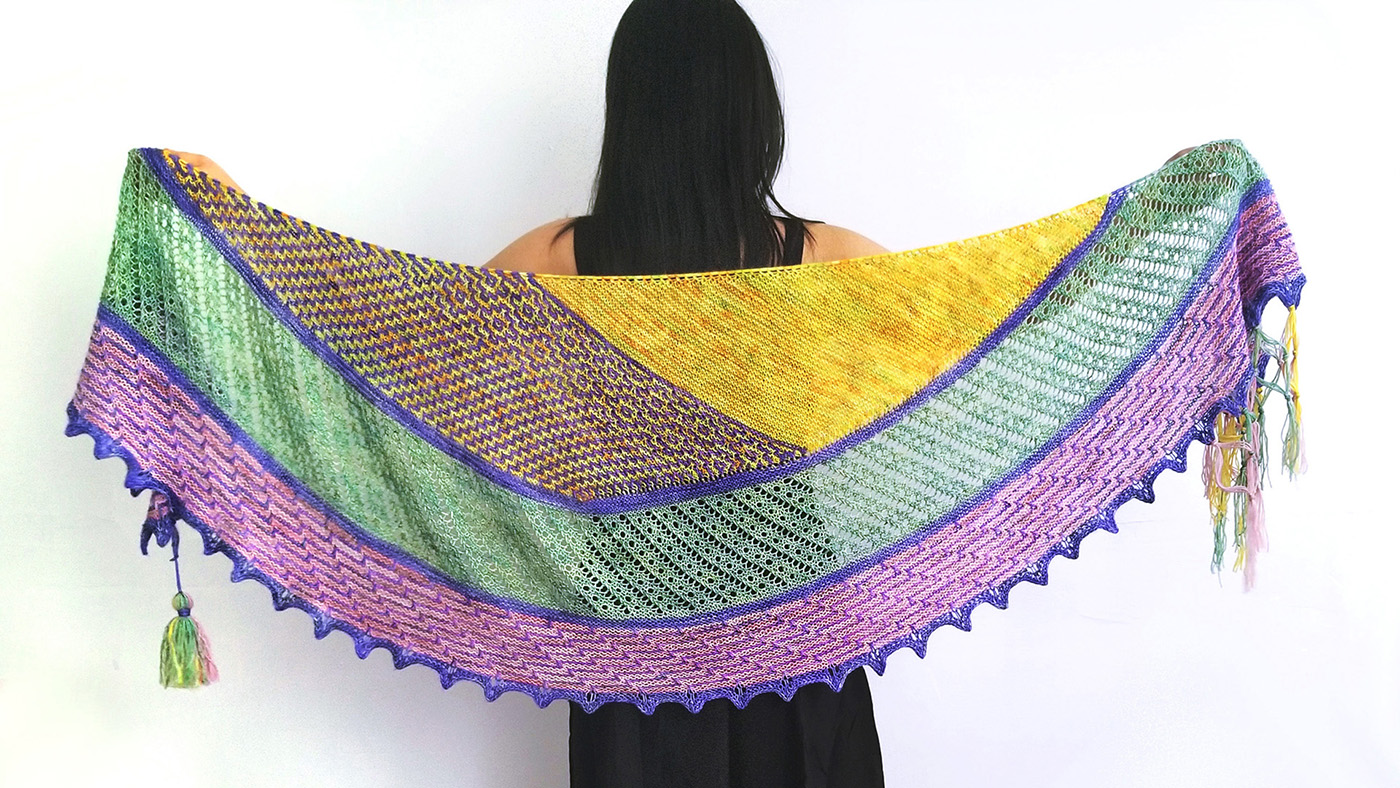
\includegraphics[width=\linewidth]{backspread-small.jpg}
\end{center}

% uncommend line below if you want a background fill image
% \ThisLRCornerWallPaper{1.0}{image.jpg} 

{\fontfamily{qag}\selectfont
\HUGE\textbf{\thetitle}
\hspace{3.5em} % adjust this space
\normalsize\theauthor
}

\begin{multicols}{2}
\small

% Cute description here
Pack your bags and hop onto the caravan! The Roulotte (``caravan" in French) shawl is an epic journey through landscapes of mosaic knitting and lace. Without any purls to slow you down, the trip will simply fly by!

\subsection*{Yarn Requirements}

% yardage, number of colors, etc.
Fingering weight yarn in 4 colors: three main colors MC1, MC2, MC3; one contrast color CC.

~\\
% also include: sample yarn, other yarn suggestions
\emph{Sample used Toad Hollow Drusilla  (superwash merino/nylon, 400yds/100g). \vspace{-.5em}
\begin{itemize}
\item 360yds CC - ``Nomad" \vspace{-.5em}
\item 180yds MC1 - ``Free Spirit" \vspace{-.5em}
\item 260yds MC2 - ``Eleutheromania" \vspace{-.5em}
\item 260yds MC3 - ``Lady Defiance" \vspace{-.5em}
\end{itemize}
Tassels used an additional 20 yds each. 
}

\subsection*{Sizing}

% sample measurements, gauge, notes on ease, etc.
% MEASURE SAMPLE WINGSPAN
One size. Sample measures 85"/216 cm from tip-to-tip and 24"/60cm deep after moderate blocking.

\vfill
\columnbreak

\subsection*{Gauge: 5 sts in 1"/2.5cm}

Gauge was measured in unblocked, unstretched garter stitch. It is not critical for the shawl, but a different gauge may change the yardage required or the size of the shawl.

\subsection*{Tools}

\begin{itemize}
\item 40" circular needle in size needed to obtain fabric of your liking. \\ \emph{Suggested size: US5/3.75mm} \vspace{-.5em}
\item tapestry needle \vspace{-.5em}
\item \emph{(optional)} cardboard for making tassels \vspace{-.5em}
\item \emph{(optional)} crochet hook for fringe \vspace{-.5em}
\end{itemize}

\subsection*{Techniques}

This pattern is suitable for an intermediate knitter. % DIFFICULTY LEVEL
Prior to knitting this pattern, you should be familiar with casting on, knitting, slipping stitches, and basic lace involving yo, k2tog, and ssk. Some support is provided for striping yarns and reading mosaic knitting charts. % PREREQUISITE TECHNIQUES
For a complete list of stitches used, see Pattern Key.

% discuss any special techniques and tutorials included

\normalsize

\subsection*{Pattern Key}

% formatting notes for charts and written directions
\vocab{Charts:} repeats = thick borders \chart{\!\underline{\overline{-}}\!}  

Charts do not show edge stitches. Follow edge instructions when using charts.

~\\
\vocab{Written instructions:} 

repeats = \textbf{*[stitches]*} to specified point
\vspace{-1em}

% stitch key - fill in with all stitches used in design: chart symbol, written abbreviation, full stitch name or explanation
% stitches with explanations must first be BOLDED, followed by colon then explanation
\begin{center}
{\renewcommand{\arraystretch}{1.5}
\begin{tabular}{| C{0.2\linewidth}  p{0.7\linewidth} | }
\thickhline \rowcolor{shadecolor} 
\textbf{Written}	& \textbf{Description} \\ \thickhline
CO 	& cast on \\
k	& knit \\
kfb 	& knit front back \\
sl 	& slip stitch purlwise; \textbf{wyib} - ``with yarn in back" or \textbf{wyif} - ``with yarn in front" \\
k2tog 	& knit 2 together \\
ssk		& slip slip knit \\
yo		& yarn-over  \\
\hline
\end{tabular}
}

\end{center}

%%%%%%%%%%%%%%%%%%%%%%%%%%%%%%%%%%%%%%%%%%%%%%%%%%
% BEGIN INSTRUCTIONS

\vfill
\columnbreak

\section*{Cast On and Set Up}

With MC1, CO 4 sts. Work Set Up Rows 1-10.

~\\
\rowDir{Row 1 (RS)} k3, kfb. \stitchcount{5}

\rowDir{Row 2 (WS)} k2, sl3 wyif.

\rowDir{Row 3} k3, kfb, k1. \stitchcount{6}

\rowDir{Row 4} k3, sl3 wyif.

\rowDir{Row 5} k3, kfb, k2. \stitchcount{7}

\rowDir{Row 6} k4, sl3 wyif.

\rowDir{Row 7} k3, kfb, k3. \stitchcount{8}

\rowDir{Row 8} k5, sl3 wyif.

\rowDir{Row 9} k3, kfb, k1, k2tog, k1

\rowDir{Row 10} k4, kfb, sl3 wyif. \stitchcount{9}

\end{multicols}

\section*{Section 1}

\rowDir{Row 11 (RS)} k3, kfb, k to 3 sts from end, k2tog, k1.

\rowDir{Row 12 (WS)} k to 4 sts from end, kfb, sl3 wyif. \increase{1}

~\\
Repeat Rows 11 and 12 an additional 70 times, ending after a WS row. 80 sts total.

\subsection*{Transition to Section 2}

Join CC. Using CC, work one more repeat of Rows 11 and 12. \increase{1} 81 sts total.


\section*{Section 2}

In Section 2, you will be striping MC1 and CC while carrying them along the edge of the work. See \textbf{Special Techniques} for notes on carrying yarn while striping and for reading mosaic charts.

\newpage
Work 2 repeats of Mosaic 1. \emph{(+12 sts per repeat)} 105 sts total.

\subsection*{Mosaic 1 Instructions}

\rowDir{Row 1 (RS, MC1)} k3, kfb, k5, \repeat{sl1 wyib, k5} to 6 sts from end, sl1 wyib, k2, ssk, k1. \\
\rowDir{Row 2 (WS, MC1)} k4, \repeat{sl1 wyif, k5} to 5 sts from end, k1, kfb, sl3 wyif. \\
\rowDir{Row 3 (CC)} k3, kfb, k2, \repeat{sl1 wyib, k3} to 4 sts from end, sl1 wyib, ssk, k1. \\
\rowDir{Row 4 (CC)} k2, \repeat{sl1 wyif, k3} to 4 sts from end, kfb, sl3 wyif. \\
\rowDir{Row 5 (MC1)} k3, kfb, k1, sl1 wyib, \repeat{k3, sl1 wyib, k1, sl1 wyib} to 5 sts from end, k2, ssk, k1. \\
\rowDir{Row 6 (MC1)} k4, \repeat{sl1 wyif, k1, sl1 wyif, k3} to 7 sts from end, sl1 wyif, k2, kfb, sl3 wyif. \\
\rowDir{Row 7 (CC)} k3, kfb, k4, \repeat{sl1 wyib, k3} to 4 sts from end, sl1 wyib, ssk, k1. \\
\rowDir{Row 8 (CC)} k2, \repeat{sl1 wyif, k3} to 6 sts from end, k2, kfb, sl3 wyif. \\
\rowDir{Row 9 (MC1)} k3, kfb, k1, \repeat{sl1 wyib, k5} to 8 sts from end, sl1 wyib, k4, ssk, k1. \\
\rowDir{Row 10 (MC1)} k6, \repeat{sl1 wyif, k5} to 7 sts from end, sl1 wyif, k2, kfb, sl3 wyif. \\
\rowDir{Row 11 (CC)} k3, kfb, k2, \repeat{sl1 wyib, k3} to 4 sts from end, sl1 wyib, ssk, k1. \\
\rowDir{Row 12 (CC)} k2, \repeat{sl1 wyif, k3} to 4 sts from end, kfb, sl3 wyif. \\
\rowDir{Row 13 (MC1)} k3, kfb, k1, \repeat{sl1 wyib, k1, sl1 wyib, k3} to 4 sts from end, sl1 wyib, ssk, k1. \\
\rowDir{Row 14 (MC1)} k2, sl1 wyif, \repeat{k3, sl1 wyif, k1, sl1 wyif} to 6 sts from end, k2, kfb, sl3 wyif. \\
\rowDir{Row 15 (CC)} k3, kfb, k2, \repeat{sl1 wyib, k3} to 6 sts from end, sl1 wyib, k2, ssk, k1. \\
\rowDir{Row 16 (CC)} k4, \repeat{sl1 wyif, k3} to 4 sts from end, kfb, sl3 wyif. \\
\rowDir{Row 17 (MC1)} k3, kfb, k3, \repeat{sl1 wyib, k5} to 4 sts from end, sl1 wyib, ssk, k1. \\
\rowDir{Row 18 (MC1)} k2, \repeat{sl1 wyif, k5} to 9 sts from end, sl1 wyif, k4, kfb, sl3 wyif. \\
\rowDir{Row 19 (CC)} k3, kfb, k4, \repeat{sl1 wyib, k3} to 6 sts from end, sl1 wyib, k2, ssk, k1. \\
\rowDir{Row 20 (CC)} k4, \repeat{sl1 wyif, k3} to 6 sts from end, k2, kfb, sl3 wyif. \\
\rowDir{Row 21 (MC1)} k3, kfb, \repeat{k3, sl1 wyib, k1, sl1 wyib} to 3 sts from end, ssk, k1. \\
\rowDir{Row 22 (MC1)} k2, \repeat{sl1 wyif, k1, sl1 wyif, k3} to 5 sts from end, k1, kfb, sl3 wyif. \\
\rowDir{Row 23 (CC)} k3, kfb, k2, \repeat{sl1 wyib, k3} to 6 sts from end, sl1 wyib, k2, ssk, k1. \\
\rowDir{Row 24 (CC)} k4, \repeat{sl1 wyif, k3} to 4 sts from end, kfb, sl3 wyif.

\subsection*{Mosaic 1 Chart}


For Mosaic 1, work i-cord selvedge along one edge as follows:

\hspace{2em} \rowDir{RS Row} k3, kfb, work chart to last 3 sts, ssk, k1.

\hspace{2em} \rowDir{WS Row} k2, work chart to last 5 sts, k1, kfb, sl3 wyif. \increase{1} \\

\small
\textknit{-} k in MC (RS and WS) \hspace{2em} \textknit{=} k in CC (RS and WS) \hspace{2em}
\textknit{v} sl1 wyib (RS); sl1 wyif (WS) \\

\chart[right]{
~~~~~~~~~\rnleft ==\!v===v===v===\!v===v===v==
~~~~~~~~\rnleft V-V\!---V-V---V-V\!---V-V---
~~~~~~~\rnleft==v=\!==v===v===v=\!==v====
~~~~~~\rnleft V----\!-V-----V----\!-V---
~~~~~\rnleft==v===\!v===v===v===\!v==
~~~~\rnleft V---V-V\!---V-V---V-V\!-
~~~\rnleft v===v===\!v===v===v===\!v===v===v==
~~\rnleft----V----\!-V-----V----\!-V-----V-
~\rnleft v===v===v=\!==v===v===v=\!==v====
\rnleft--V-V---V-V\!---V-V---V-V\!---V-
~~~~~~~~~~~\rnleft\!v===v===v===\!v==
~~~~~~~~~~\rnleft-\!-V-----V----\!-
}
\normalsize \newpage

Then, work 5 repeats of Mosaic 2. \emph{(+4 sts per repeat)} 125 sts total.

\subsection*{Mosaic 2 Instructions} % add edge sts

\rowDir{Row 1 (RS, MC1)} k3, kfb, k1, \repeat{sl1 wyib, k3} to 4 sts from end, sl1 wyib, ssk, k1. \\
\rowDir{Row 2 (WS, MC1)} k2, \repeat{sl1 wyif, k3} to 7 sts from end, sl1 wyif, k2, kfb, sl3 wyif. \\
\rowDir{Row 3 (CC)} k3, kfb, k4, \repeat{sl1 wyib, k3} to 6 sts from end, sl1 wyib, k2, ssk, k1. \\
\rowDir{Row 4 (CC)} k4, \repeat{sl1 wyif, k3} to 6 sts from end, k2, kfb, sl3 wyif. \\
\rowDir{Row 5 (MC1)} k3, kfb, k3, \repeat{sl1 wyib, k3} to 4 sts from end, sl1 wyib, ssk, k1. \\
\rowDir{Row 6 (MC1)} k2, \repeat{sl1 wyif, k3} to 5 sts from end, k1, kfb, sl3 wyif. \\
\rowDir{Row 7 (CC)} k3, kfb, k2, \repeat{sl1 wyib, k3} 6 sts from end, sl1 wyib, k2, ssk, k1. \\
\rowDir{Row 8 (CC)} k4, \repeat{sl1 wyif, k3} to 4 sts from end, kfb, sl3 wyif. 

\subsection*{Mosaic 2 Chart}

For Mosaic 2, work i-cord selvedge along one edge as follows:

\hspace{2em} \rowDir{RS Row} k3, kfb, work chart to last 3 sts, ssk, k1.

\hspace{2em} \rowDir{WS Row} k2, work chart to last 5 sts, k1, kfb, sl3 wyif. \increase{1}

\begin{multicols}{2}

\chart[right]{
\rnleft ==v\!===v\!==
~~~\rnleft \!V---\!
~~\rnleft =\!=v==\!==
~\rnleft V-\!--V-\!
}

\vfill
\columnbreak
\small
\textknit{-} k in MC (RS and WS) \\ 

\textknit{=} k in CC (RS and WS) \\

\textknit{v} sl1 wyib (RS); sl1 wyif (WS)

\end{multicols}

\subsection*{Transition to Section 3} 

Break MC1. Working in CC,

\rowDir{Next RS row} k3, kfb, k to end. \increase{1} At the end of the row, do not turn work. Instead, with RS facing, pick up and knit 1 st from every garter ridge on the left selvedge, of which there should be 120. When you reach the CO corner of the piece, turn to WS. 
\\ \increase{120} 246 sts total. \\
\rowDir{Next WS row} Pick up and knit 3 sts in CO edge of the i-cord border as shown below.  K to 4 sts from end, kfb, sl3 wyif. \increase{4} 250 sts total.

\begin{center}
\vspace{-2em}
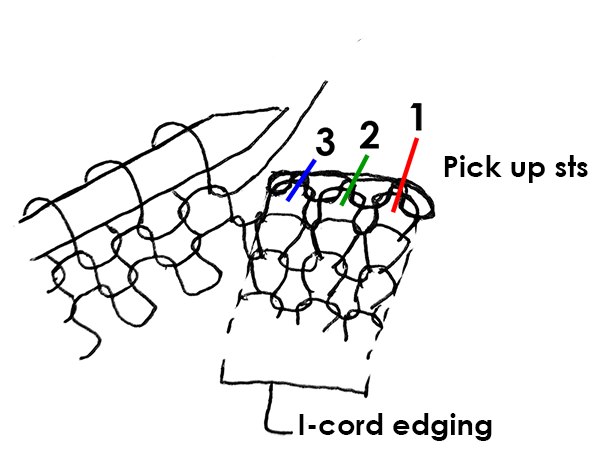
\includegraphics[height=2in]{pickup.png}
\end{center}

Continuing in CC, work 4 repeats of the following Garter Row to create 2 garter ridges. 

\rowDir{Garter Row (RS and WS)} k3, kfb, k to last 4 sts, kfb, sl3 wyif. \increase{2}

~\\
Break CC. Join MC2 and work 2 repeats of the Garter Row. 262 sts total. 

\newpage
\section*{Section 3} % increase 84

You should begin this section with a multiple of 6 plus 4 sts. Continuing in MC2, work 3 repeats of Lace. \emph{(+24 sts per repeat)} 334 sts total.

~\\
Then, work Rows 1-6 of Lace once more. \increase{12} 346 sts total.


\subsection*{Lace Instructions} % add edge sts

\rowDir{Row 1 (RS)} k3, kfb, \repeat{yo, k2tog, k4} to 6 sts from end, yo, k2tog, kfb, sl3 wyif. \\
\rowDir{Row 2 (WS)} k3, kfb, k1, \repeat{sl1 wyif, k5} to 7 sts from end, sl1 wyif, k2, kfb, sl3 wyif. \\
\rowDir{Row 3} k3, kfb, \repeat{yo, k2tog, k1} to 4 sts from end, kfb, sl3 wyif. \\
\rowDir{Row 4} k3, kfb, k2, \repeat{sl1 wyif, k5} to 4 sts from end, kfb, sl3 wyif. \\
\rowDir{Row 5} k3, kfb, \repeat{yo, k2tog, k4} to 8 sts from end, yo, k2tog, k2, kfb, sl3 wyif. \\
\rowDir{Row 6} k3, kfb, k3, \repeat{sl1 wyif, k5} to 7 sts from end, sl1 wyif, k2, kfb, sl3 wyif. \\
\rowDir{Row 7} k3, kfb, \repeat{yo, k2tog, k1} to 6 sts from end, yo, k2tog, kfb, sl3 wyif. \\
\rowDir{Row 8} k3, kfb, k4, \repeat{sl1 wyif, k5} to 4 sts from end, kfb, sl3 wyif. \\
\rowDir{Row 9} k3, kfb, \repeat{yo, k2tog, k4} to 4 sts from end, kfb, sl3 wyif. \\
\rowDir{Row 10} k3, kfb, k5, \repeat{sl1 wyif, k5} to 7 sts from end, sl1 wyif, k2, kfb, sl3 wyif. \\
\rowDir{Row 11} k3, kfb, \repeat{yo, k2tog, k1} to 5 sts from end, k1, kfb, sl3 wyif. \\
\rowDir{Row 12} k3, kfb, k6, \repeat{sl1 wyif, k5} to 4 sts from end, kfb, sl3 wyif.

\subsection*{Lace Chart}

For Lace, work i-cord selvedge along both edges as follows:

\hspace{2em} \rowDir{RS Row} k3, kfb, work chart to last 4 sts, kfb, sl3 wyif. \increase{2}

\hspace{2em} \rowDir{WS Row} k3, kfb, k1, work chart to last 5 sts, k1, kfb, sl3 wyif. \increase{2}

\begin{multicols}{2}
\chart[oddright]{
-----v\!-----v\!----
-->O->\!O->O->\!O->O
~~----\!v-----\!v-
~~----\!>O----\!>O
~~~~--\!-v----\!
~~~~>O\!->O->O\!
~~~~~~\!--v---\!--v-
~~~~~~\!-->O--\!-->O
~~-v--\!---v--\!--
~~->O-\!>O->O-\!>O
~~~~v-\!----v-\!
~~~~>O\!---->O\!
}

\vfill \columnbreak
\begin{addmargin}[4em]{0em} \small

\textknit{-} k (RS and WS) \\

\textknit{v} sl1 wyif \\

\textknit{O} yo \\

\textknit{>} k2tog
\end{addmargin}
\end{multicols}

\subsection*{Transition to Section 4} % increase 16 (4 garter ridges) for 362 sts

Work Garter Row twice in MC2. Break MC2, join CC. Work Garter Row six times in CC. 
\\ \increase{16} 362 sts total.

\newpage
\section*{Section 4} % start with 362

Join MC3. In Section 4, you will be striping MC3 and CC while carrying them along the edge of the work. You should begin Section 4 with a multiple of 8 plus 2 sts. 

~\\
Work 4 repeats of Mosaic 3. \emph{(+24 sts per repeat)} 458 sts total.

~\\
Work Rows 1-4 of Mosaic 3 again. \increase{8} 466 sts total or 56 elongated slip sts from Mosaic 3.

\subsection*{Mosaic 3 Instructions} % add edge sts

\rowDir{Row 1 (RS, MC3)} k3, kfb, k7, \repeat{sl1 wyib, k7} to 7 sts from end, sl1 wyib, k2, kfb, sl3 wyif. \\
\rowDir{Row 2 (WS, MC3)} k3, kfb, k3, \repeat{sl1 wyif, k7} to 5 sts from end, k1, kfb, sl3 wyif. \\
\rowDir{Row 3 (MC3)} k3, kfb, k9, \repeat{sl1 wyib, k7} to 9 sts from end, sl1 wyib, k4, kfb, sl3 wyif. \\
\rowDir{Row 4 (MC3)} k3, kfb, k5, \repeat{sl1 wyif, k7} to 7 sts from end, k3, kfb, sl3 wyif. \\
\rowDir{Row 5 (CC)} k3, kfb, k4, \repeat{sl1 wyib, k7} to 10 sts from end, sl1 wyib, k5, kfb, sl3 wyif. \\
\rowDir{Row 6 (CC)} k3, kfb, k6, \repeat{sl1 wyif, k7} to 10 sts from end, sl1 wyif, k5, kfb, sl3 wyif. \\
\rowDir{Row 7 (MC3)} k3, kfb, k7, \repeat{sl1 wyib, k7} to 11 sts from end, sl1 wyib, k6, kfb, sl3 wyif. \\
\rowDir{Row 8 (MC3)} k3, kfb, k7, \repeat{sl1 wyif, k7} to 5 sts from end, k1, kfb, sl3 wyif. \\
\rowDir{Row 9 (MC3)} k3, kfb, k9, \repeat{sl1 wyib, k7} to 5 st from end, k1, kfb, sl3 wyif. \\
\rowDir{Row 10 (MC3)} k3, kfb, k9, \repeat{sl1 wyif, k7} to 7 sts from end, k3, kfb, sl3 wyif. \\
\rowDir{Row 11 (CC)} k3, kfb, k4, \repeat{sl1 wyib, k7} to 6 sts from end, sl1 wyib, k1, kfb, sl3 wyif. \\
\rowDir{Row 12 (CC)} k3, kfb, k2, \repeat{sl1 wyif, k7} to 10 sts from end, sl1 wyif, k5, kfb, sl3 wyif. 

\subsection*{Mosaic 3 Chart}

For Mosaic 3, work i-cord selvedge along both edges as follows:

\hspace{2em} \rowDir{RS Row} k3, kfb, work chart to last 4 sts, kfb, sl3 wyif. \increase{2}

\hspace{2em} \rowDir{WS Row} k3, kfb, k1, work chart to last 5 sts, k1, kfb, sl3 wyif. \increase{2}

\begin{multicols}{2}
\chart[right]{
~~\rnleft=v==\!=====v==\!==
~~~~\rnleft--\!------V-\!--------
~~~~~~\rnleft\!------V-\!------
\rnleft=====v\!=======v\!====
~~\rnleft----\!V-------\!--
~~~~\rnleft--\!V-------\! % 8n+2
}

\vfill \columnbreak

\begin{addmargin}[8em]{0em} \small
\textknit{-} k in MC (RS and WS) \\ 

\textknit{=} k in CC (RS and WS) \\

\textknit{v} sl1 wyib (RS); sl1 wyif (WS)
\end{addmargin}

\end{multicols}

\newpage

\begin{frnote}
\textbf{Modification Suggestions:} If you are running low on CC for the final section, you might:
\begin{itemize} \small
\item Only work Rows 1-3 then skip to bind-off. 
\item Work all rows and bind-off, but mix stripes of CC, MC1, MC2, and/or MC3. 
\item Stripe the i-cord bind-off. \vspace{-1em}
\end{itemize}
\end{frnote}

\section*{Final Section and Bind Off}

Break MC3. Continuing in CC, work the following rows:

\rowDir{Row 1 (RS)} k3, kfb, k to last 4 sts, kfb, sl3 wyif. \increase{2} \\
\rowDir{Row 2 (WS)} k3, kfb, k7 (the next stitch should be above an elongated slip st), \repeat{yo, kfb, yo, k7} to 9 sts from end, k5, kfb, sl3 wyif. \\ (\emph{increased 2 + 3(56) = 170 sts})\\
\rowDir{Row 3} k3, kfb, k to last 4 sts, kfb, sl3 wyif. \\ \increase{2} \\
\rowDir{Row 4} k3, kfb, k10, \repeat{yo, k1, yo, k1, yo, k9} to 10 sts from end, k6, kfb, sl3 wyif. \\ (\emph{increased 2 + 3(56) = 170 sts}) \\
\rowDir{Row 5} k3, kfb, k to last 4 sts, kfb, sl3 wyif. \\ \increase{2}

812 sts total.


~\\
Turn work to WS and work 4 rounds of i-cord as follows:

\rowDir{I-cord} K 3 sts. Keeping yarn in back, slip the 3 sts on R needle back to the L needle.

~\\
Bind-off sts on WS as follows, until there are 6 sts left on the needle.

\rowDir{I-cord Bind-off} k2, k2tog. Keeping yarn in back, slip the 3 sts on R needle back to the L needle. \decrease{1}

~\\
At the end of the bind-off, work 3 rounds of i-cord, then graft the first 3 sts to the last 3 sts as shown below.

\vspace{-1em}
\begin{center}
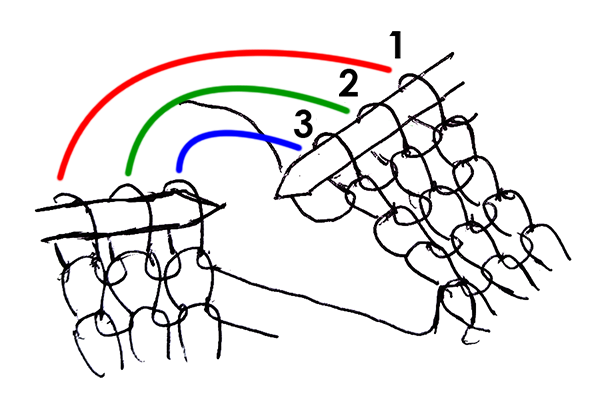
\includegraphics[height=2in]{kitchener.png}
\end{center}

\vspace{-4em}
\section*{Finishing}

Block shawl, taking care to pin out each scallop of the final section. Weave in all ends.

~\\
If desired, attach tassels or fringe as suggested in \textbf{Special Techniques}.


\newpage
%%%%%%%%%%%%%%%%%%%%%%%%%%%%%%%%%%%%%%%%%%%%%%%%%%
% APPENDICES (IF ANY)
\begin{multicols}{2}
\section*{Special Techniques}

\subsection*{Striping Yarns}

When working the mosaic patterns, you will only use one color at a time and leave the other hanging on the end of your row. When you switch colors at the beginning of a row, drop the old color, then pick up the new color from underneath the old color to lock in the hanging yarn.

\subsection*{Reading Mosaic Charts}

In this particular compact style of mosaic chart, I have compressed two rows of knitting into one charted row. Each row of the chart should be read twice: once from right to left, then again from left to right. For further information on mosaic charts, refer to this \href{https://www.interweave.com/article/knitting/tech-tip-mosaic-knitting/}{\underline{\emph{Interweave article.}}}

\subsection*{Making Tassels}

Use any selection of MC1, MC2, MC3, and/or CC to make your tassels.

\begin{enumerate}
\item Wrap yarn 60 times (or to desired density) around a piece of cardboard approx. 6"/15cm wide.
\item Cut an 8"/20cm length of yarn to tie the loops together at the top of the cardboard, using a tight double knot.
\item Cut the loops at the bottom of the card to create the bottom of the tassel.
\item Create the head of the tassel using another 8"/20cm length of yarn to wrap around the top of the tassel and weaving in the ends.
\item Trim ends to an even length.
\item Attach tassel to the bind-off corner loops using the ties.
\end{enumerate}

\vfill
\begin{center}
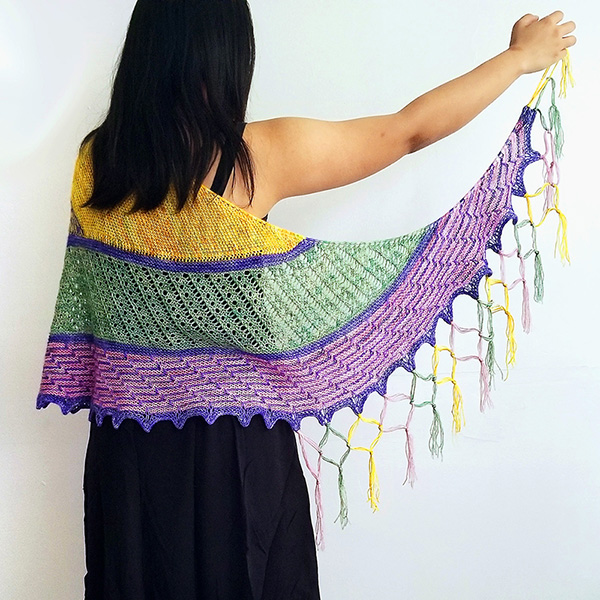
\includegraphics[width=.9\linewidth]{macrame.jpg}
\end{center}

\subsection*{Attaching Macrame Fringe}

Use any selection of MC1, MC2, MC3, and/or CC to make fringe. For example, you might use MC1, MC2, and MC3 in a repeating sequence.

\begin{enumerate}
\item Create 58 bundles of yarn for each scallop of the edge (including the loops at the beginning and end), each having five 2ft/60cm lengths of yarn.
\item Fold each bundle in half to create a loop at one end. Using a crochet hook, hook loop through an eyelet on the edge, then pull the loose ends through to tie a lark's head knot. Each fringe bundle should have 10 ends of yarn.
\item Taking 5 ends from one bundle and 5 ends from the bundle next to it, tie them together in an overhand knot approx. 2"/5cm from the lark's head knot. Repeat across the shawl, leaving 5 ends on the first and last bundles loose.
\item Take the 5 loose ends from the first bundle and 5 ends from the next bundle, then tie them together in an overhand knot approx. 2"/5cm from the previous overhand knot. Repeat across the shawl to form diamonds.
\end{enumerate}
\vfill
~
\end{multicols}

\end{document}